\section{System to Build} \label{sec:promise}

%P1 introduce the two components we want to build
\Name's main components includes a container locator and a virtualized NIC.
The container locator can figure out where the location of the container is and
decide the most efficient way for two containers to talk with each other.
And the virtualized NIC emulates the necessary underlying resource structures 
(e.g., send queue or receive queue of the NIC). In this way, the application will
be using the standardized APIs without be aware of the actual communication
mechanisms.

\begin{itemize}
  \item Container Locator:
  \item Virtualized NIC:
\end{itemize}

     \begin{figure}[ht]
     \centering 
     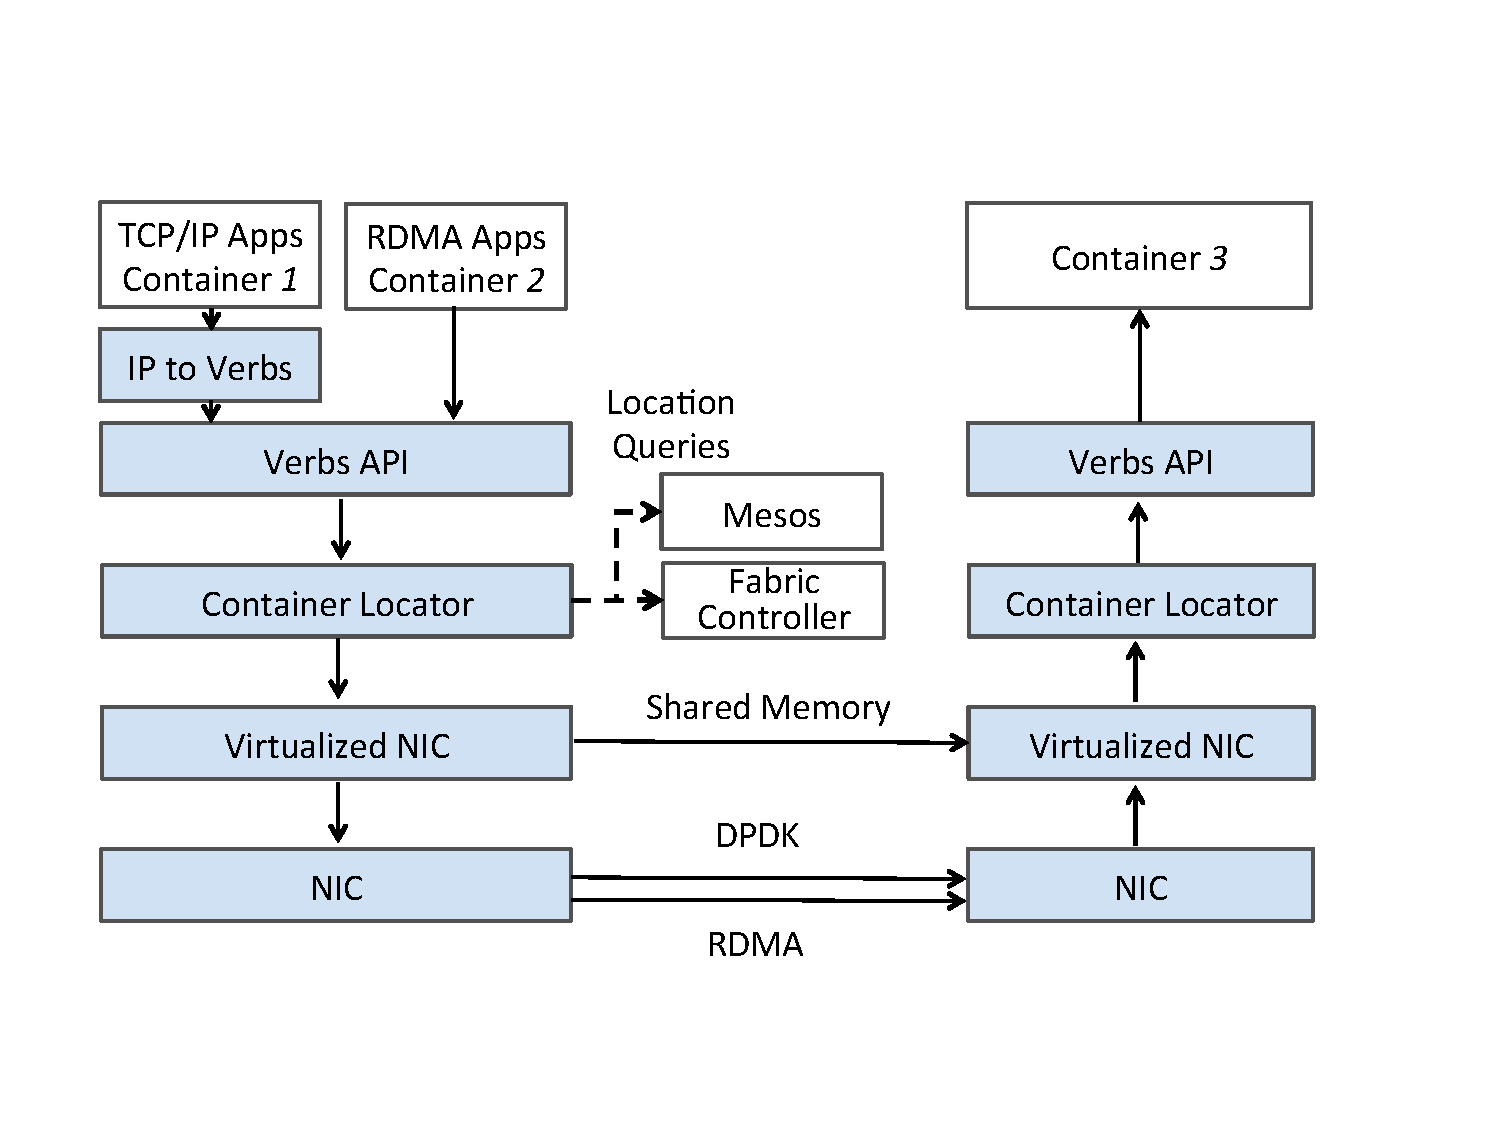
\includegraphics[width=0.5\textwidth]{figures/system/system_modules.pdf}      
     \label{fig:system_modules}
     \caption{The system modules.} 
     \end{figure}